% arara: xelatex
% arara: xelatex
% arara: xelatex

% options:
% thesis=B bachelor's thesis
% thesis=M master's thesis
% czech thesis in Czech language
% english thesis in English language
% hidelinks remove colour boxes around hyperlinks

\documentclass[thesis=M,english]{prefs/FITthesis}[2019/03/06]

% \usepackage{subfig} %subfigures
% \usepackage{amsmath} %advanced maths
% \usepackage{amssymb} %additional math symbols

\usepackage[utf8]{inputenc}

\usepackage{graphicx} %graphics files inclusion
% \usepackage{amsmath} %advanced maths
% \usepackage{amssymb} %additional math symbols

\usepackage{dirtree} %directory tree visualisation
\usepackage{subfig} %image side by side
\usepackage{todonotes} %todo
\usepackage{url}
\usepackage{textcomp} %degree symbol
\usepackage{color, colortbl} %color, table color
\usepackage{enumitem} %lists
\usepackage{float} %for H option in figures
\usepackage{array} %table aligment       
\usepackage{amsmath} %cases
\usepackage{svg} %svg
\usepackage{scrextend}
\usepackage{multirow}
\addtokomafont{labelinglabel}{\sffamily}


% list of acronyms
\usepackage[acronym,nonumberlist,toc,nopostdot,numberedsection=autolabel,nomain]{glossaries}
\makeglossaries
\newcommand{\tg}{\mathop{\mathrm{tg}}} %cesky tangens
\newcommand{\cotg}{\mathop{\mathrm{cotg}}} %cesky cotangens

% % % % % % % % % % % % % % % % % % % % % % % % % % % % % % % % % % % 
% % % % % % % % % % % % % % % % % % % % % % % % % % % % % % % % % % % 
\department{Department of Applied Mathematics}
\title{People detection, tracking and biometric data extraction using a single camera for retail usage}
\authorGN{Luk{\' a}{\v s}} %author's given name/names
\authorFN{Brchl} %author's surname
\authorWithDegrees{Bc. Luk{\' a}{\v s} Brchl} %author's name with academic degrees
\author{Luk{\' a}{\v s} Brchl} %author's name without academic degrees
\supervisor{doc. RNDr. Ing. Marcel Jiřina, Ph.D.}
\acknowledgements{}
\abstractCS{}
\abstractEN{This thesis aims to design and implement a framework that analyzes video sequences to extract as much information as possible about the people in the scene captured by a single RGB camera. The whole framework can be broken down into the smaller components, i.e. people detector, people tracker. and biometrics extractor. The people detector employs a well-known deep-learning architecture to estimate bounding boxes of individuals. The tracking solution is built to be robust regarding the crowded scenes by incorporating multiple features in matching phase such as person's visual appearance, motion, face, and height. Each new detection has these features calculated by various computer vision algorithms and then these hypotheses are matched against existing tracks utilizing multiple distance metrics. Apart from using the features only for matching, they are kept for calculation of various output statistics. The approach is validated against the dataset which was created for this propose. The integration of face information in matching phase greatly improves the performance, however it is not always possible to extract it. This face information also helps to maintain a person identity even when when they leave the scene and then reappears. At the end, it is shown what the output statistics can be used for.}
\placeForDeclarationOfAuthenticity{} %where you have signed the declaration
\keywordsCS{počítačové vidění, detekce osob, sledování osob, extrakce biometrických údajů}
\keywordsEN{computer vision, people detection, people tracking, biometrics extraction}
\declarationOfAuthenticityOption{5} %select as appropriate, according to the desired license
\website{https://github.com/lukasbrchl/People-detection-tracking-and-biometrics-extraction-using-a-single-camera-text} %optional URL (remove entirely if you have no URL for this thesis)

%introduction
\newacronym{gpu}{GPU}{graphics processing unit}
\newacronym{mot}{MOT}{multiple object tracking}
\newacronym{mtmct}{MTMCT}{multi-target multi-camera tracking}
\newacronym{reid}{ReID}{re-identification}
%theoretical backround
\newacronym{ai}{AI}{artificial intelligence}
\newacronym{ml}{ML}{machine learning}
\newacronym{pca}{PCA}{principal component analysis}
\newacronym{dl}{DL}{deep learning}
\newacronym{cv}{CV}{computer vision}
\newacronym{ann}{ANN}{artificial neural network}
\newacronym{nn}{NN}{neural network}
\newacronym{mlp}{MLP}{multi layer perceptron}
\newacronym{cnn}{CNN}{convolutional neural network}
\newacronym{svm}{SVM}{support vector machine}
\newacronym{lbp}{LBP}{local binary pattern}
\newacronym{hog}{HOG}{histogram of oriented gradients}
\newacronym{sift}{SIFT}{Scale-invariant feature transform}
\newacronym{surf}{SURF}{Speeded-Up Robust Features}
\newacronym{r-cnn}{R-CNN}{region-based convolutional network}
\newacronym{fast r-cnn}{Fast R-CNN}{fast region-based convolutional network}
\newacronym{faster r-cnn}{Faster R-CNN}{faster region-based convolutional network}
\newacronym{rpn}{RPN}{region proposal network}
\newacronym{yolo}{YOLO}{you only look once}
\newacronym{nms}{NMS}{non-maximum suppression}
\newacronym{ssd}{SSD}{single-shot detector}
\newacronym{fps}{FPS}{frames per second}
%related work
\newacronym{mots}{MOTS}{multiple object tracking and segmentation}
\newacronym{sort}{SORT}{simple online and real-time tracking}
\newacronym{rnn}{RNN}{recurrent neural network}
\newacronym{lstm}{LSTM}{long short-term memory}

\begin{document}
    \begin{introduction}
    Detection of people and their subsequent identity preservation in a video sequence (tracking) is a part of a more broader domain task called \gls{mot}. In the basic definition, \gls{mot} tries to estimate the position of the objects from multiple predefined classes, and then maintain their identity through the whole video sequence. 
    
    In most cases, position estimation is done by a component known as the object detector, which predicts the bounding boxes with real-valued confidences of each object class in each video frame. However, the conventional object detector does not guarantee the relationship between objects in consecutive frames. Therefore, it is necessary to extract additional features from each detected object to build the relationship in the sequence of frames. 
    
    The extracted features are mainly based on a visual appearance, movement, and interactions of the object, but complementary information such as camera calibration and known scene parameters can also be incorporated. The subsequent tracking is then achieved by matching detected objects to preserved tracks based on various distance metrics that are calculated between features of the detected objects in a current frame and features of traced objects from previous frames. This approach is also known as online tracking-by-detection which means that only current and previous frame information is available to the tracker, in contrast with offline-based tracking where information from the whole sequence can be used at any time. 
    
    One of the tracking benefits is that we can recover the trajectories of the objects that appeared in the video sequence, based on which we can calculate various spatial statistics that can help us to improve existing processes. For example, statistics about the movement within waiting halls might be helpful for companies to improve their indoor space and arrangement. 
    
    Even though this thesis focuses only on the task of people tracking, we may still apply many principles from more general \gls{mot}. A follow-up step after successfully building the people tracking framework is the extraction of additional class-specific information about people (soft-biometrics). This estimated data can be utilized in many applications from the retail environment; for example, we can utilize them in a retail store where there is the high demand for learning customer trends in specific days and hours, which could be easily achieved by collecting customer information such as age, gender, mood, etc. Other scenarios could be with a personalized advertisement targeted at passers-by in a shopping center or real-time staff alert when senior enters a store to offer immediate assistance. Moreover, we could use this framework to distinguish between customers and employees so we can analyze their interaction or even go further and optimize the distribution of employees around the store.
    
    \section{Motivation}
        \gls{mot} is one of the essential topics in the computer vision field. A large number of surveillance cameras in use has led to strong demand for automatic methods of processing their outputs. For example in the field of crowd image analysis, the scientific challenge is to devise and implement methods for obtaining detailed information about the number, density, movements, and actions involving people observed by a single camera or by a network of cameras.  
        
        Historically, the progress in \gls{mot} field has been limited by the number and size of the available datasets, and it was especially challenging to make comparisons between algorithms if they have been tested on different datasets under widely varying conditions. Thus, the needs of the researchers eventually formed the very first and most known PETS2009 \cite{ferryman2009pets2009} person tracking dataset. However, this dataset is minimalist. There are only three sequences related to the person tracking with ground-truth information, and evaluation metrics were often applied inconsistently, for example involving using different subsets of the available data, different ways of training the models, or differing evaluation scripts \cite{MOTChallenge2015}.
        
        The big break came in the year 2015 when MOTChallenge \cite{MOTChallenge2015} was released with the goal of standardization of quantitative benchmark to address such issues. Not only did they create unified evaluation framework with standardized metrics, but they also created the large-scale dataset with a total of 22 sequences, half for training and a half for testing purpose, with a total of 11286 frames or 996 seconds of video. This benchmark has massively transformed the \gls{mot} field which resulted in severe improvements to existing algorithms. Its popularity can also be expressed in numbers; for example, 99 \gls{mot} tracking algorithms were submitted to the MOT17 challenge \cite{mot16} during the year 2017 and similarly previous years. 
        
        Since the accuracy of existing algorithms is increasing and the price of \gls{gpu} computations is decreasing, new and more challenging datasets are being invented. VisDrone2018 \cite{zhuvisdrone2018} is a current state-of-the-art \gls{mot} dataset with over 260 video clips and more than 2.5 million bounding boxes of various class objects annotated. The frames are captured by several drone-mounted cameras which causes an unusual perspective and makes the dataset even more challenging. 
        
        To this date, there are more than ten large-scale \gls{mot} benchmarks publicly available which demonstrates that this task, especially with objects such as people, vehicles, and bicycles, has enormous attention in the research community and because the datasets are still updated to be more challenging, there are still places to improve. 
        
        The logical extension beyond detection and tracking horizons is the extraction of additional class-specific features. If we would track cars, we could take advantage of estimation of car paint, brand, and type. This information can then be used for various temporal and regional statistics; for example, for estimating the richness of a town by counting luxury-type cars. 
        
        If we take another case, which is the extraction of class-specific features about people, we could estimate attributes such as race, gender, height, mood, hair color, and clothes color. These traits are called soft-biometrics, and they are frequently used in cases where we need to complement primary biometric identifiers, such as fingerprint, palm veins, iris pattern, to provide authentication based on the unique identification of the person. The estimation of any class-specific feature is noisy. Therefore, it is essential to have reliable \gls{mot} framework, so the features are not collected from a single frame, but appropriately calculated from the whole tracking session.
        
        Although soft-biometric characteristics lack the distinctiveness and permanence to recognize an individual uniquely and reliably and can be easily faked, they provide some evidence about the people identity that could be beneficial \cite{wiki:biometrics}. With the use of soft-biometrics, we can differentiate individuals in surveillance video where it is ubiquitous that people are often occluded. In other words, despite the fact they are unable to individualize a subject, they are useful in distinguishing between people, thus maintaining people's identity in a surveillance scene. Another useful utilization is in the retail environment where we can build aggregated statistics such as the number of women between age 25 and 40 visited our store in the morning. If we have such information that in the morning there is 75 \% women of visitors, we could utilize this and adapt the store to be more suitable for women, and therefore we will have a better chance to increase profit.
        
        Last but not least, having an accurate and flawless \gls{mot} framework is crucial for further expansion to popular \gls{mtmct} field, which is the problem of determining who is where at all times given a set of video streams as input. The output of this task is also a set of person trajectories but from a wider area. Person \gls{reid} is a closely related problem in this field. Given a query image of a person, the goal is to retrieve from a database of images taken by different cameras the images where the same person appears. \cite{ristani2016MTMC}
        
    \section{Challenges}
        \gls{mot} field is deeply explored -- many methods have been proposed, and many surveys have been conducted \cite{luo2014multiple, fan2016survey, emami2018machine}. However, it is still considered as not successfully solved computer vision task. In other words, a saturation point has not yet been reached.
        
        \gls{mot} task is an extension of object detection from single images to video sequence. 
        The main challenges when using an object detector for tracking are that the resulting output is unreliable and sparse, i.e., detectors only deliver a discrete set of responses and usually yield false positives and false negatives (missing detections) as shown in Fig \ref{fig:false positive and false negative}. So, in addition to such object detection errors, identity switches are frequent in any \gls{mot} framework (see Fig. \ref{fig:id switch example}). 
    
        \begin{figure}[ht]
          \centering
          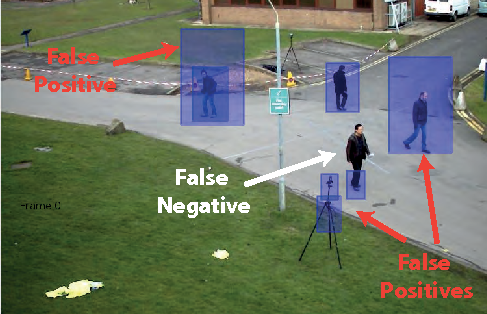
\includegraphics[width=0.7\textwidth]{resources/false-positive_and_false_negative.png}
          \caption{Example of false positive and false negative person detection. Source: \cite{yao2012interactive}.}
          \label{fig:false positive and false negative}
        \end{figure}
        
        \begin{figure}[ht]
          \centering
          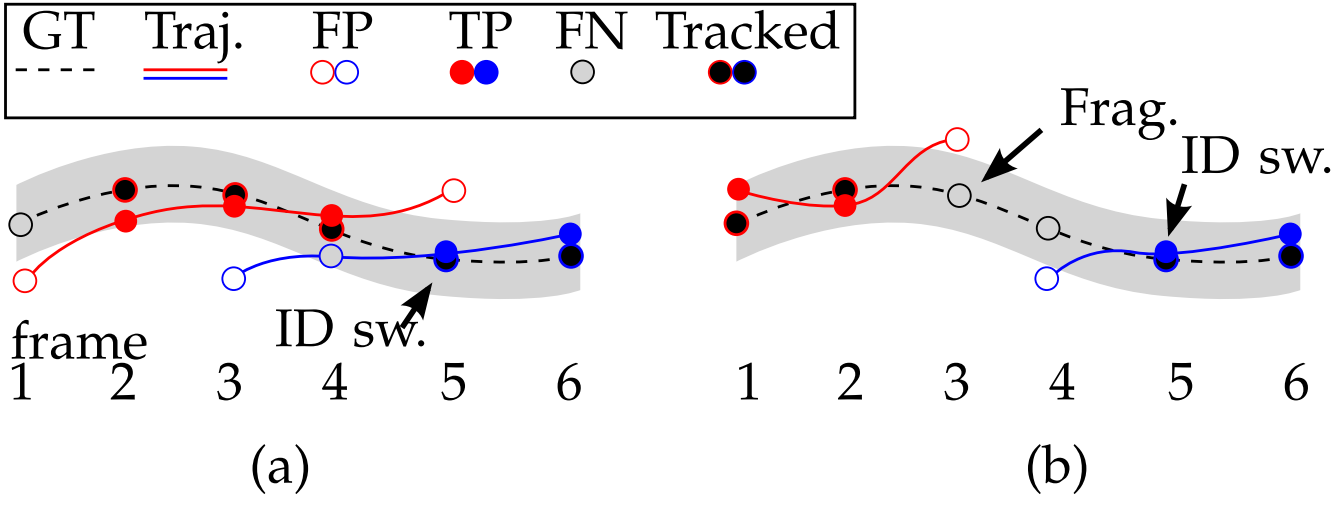
\includegraphics[width=0.7\textwidth]{resources/tracking_errors.png}
          \caption{Cases illustrating tracker-to-target assignments errors. (a) An ID switch occurs when the mapping switches from the previously assigned red track to the blue one. (b) A track fragmentation is counted in frame 3 because the target is tracked in frames 1 and 2, then interrupts, and then reacquires its ‘tracked’ status at a later point. A new (blue) track hypothesis also causes an ID switch at this point. Source: \cite{MOTChallenge2015}}
          \label{fig:id switch example}
        \end{figure}
        
        ID switches occur when there are two object trajectories are produced for one ground-truth object. Fragmentation occurs when there are two trajectories are produced with a time gap between them for one ground truth object, which implies that detections are missed in several frames. In theory, the robust tracker should handle both of these flaws. It should fill gaps in detections by propagating information from neighboring frames, and it should also filter false positive detections based on the information from previous frames. 
        
        However, it has been found out during multiple object tracking challenges that in practice, it is not entirely so. For example, in \gls{mot} \cite{mot16} dataset from 2016, 18 \% of tracks are not covered by detections at all, and 37 \% percent of tracks are covered only by low confidence of detections. When there is no high-quality detection for particular ground-truth track, then the tracker cannot resolve this problem at all, which implies that tracker usually reduces only false positives and raise false negatives by removing low-confidence detections. Nowadays, many researchers state that a robust object detector is a key to good tracking \cite{mot16, konushin2017, bewley2016simple} and during recent work \cite{luo2014multiple, fan2016survey, DBLP:journals/corr/abs-1903-05625}, it has been shown that modern object detectors can locate object even in complex, crowded scenes. However, false positives have remained frequent. 
        
        If we narrow down to the tracking people, it is even more difficult because they are very dynamic objects. People tend to change position, direction, and posture often, but they also have different height and body proportions. In real-world scenes, long-term occlusions are also frequent. As a result, it is vital for people tracking systems to be flexible so that it can handle as many different situations as possible.  
        
        Lastly, it is a topic from computer vision field where most of the work is done over images represented by matrices. It is well known that working with images is computationally demanding because each change needs to be applied for each pixel and although the image algorithms can be well parallelized, we still need to keep in mind the computation costs. 
    
    \section{Objectives}
        The goal of this thesis is to design and implement a sophisticated framework that could utilize surveillance sequences for people online tracking followed by the extraction of as much data as possible about the people in the scene, which is a three-step process. First, we need effectively and precisely acquire people detections in each frame. Then, we need to utilize a robust tracking algorithm that will maintain people identities. Lastly, gathered data from people tracking sessions must be appropriately processed for useful output statistics.
    
    \section{Assumptions}   
        The detection and tracking of people in surveillance footage is a broad topic. For this reason, the work is limited only to the one static camera watching a known scene. We assume that the captured scene is entirely under our control which means we can make any measurements and calibrate the camera. Moreover, we take into account the requirements for online processing so that the framework can be improved for real-time inference in the future. 
    
    \section{Thesis structure}
        The rest of this thesis is organized as follows. In the first chapter, we present a theoretical background which is crucial for the understanding of solving this task. Chapter 2 is devoted to the related work. Algorithm design and proposals are presented in chapter 3. Implementation details are explained in chapter 4, followed by the evaluation presented in chapter 5. The whole work is wrapped up in the last Conclusion chapter.
    
\end{introduction}
    \chapter{Theoretical background}
    This chapter provides a necessary theoretical background. We start with a general overview of artificial intelligence areas, emphasizing the computer vision field and its approaches with follow-up tasks. Lastly, we try to address the metrics needed to evaluate the algorithms used in the thesis. A reader who is familiar with the thesis topic can continue straight to the next chapter.

\section{Relevant areas}
    In this section, we go through a brief explanation of topics such as artificial intelligence, machine learning, deep learning, and computer vision. The reason for this is that many people consider these terms as effectively synonymous, but it is not so.
    
    \subsection{Artificial intelligence}
        \Gls{ai} is an area of computer science that emphasizes the creation of intelligent machines that work and react like humans. The main characteristic is that, unlike traditional algorithms, the algorithms of artificial intelligence are capable of learning from new and past data. They can enhance themselves by learning new strategies, or they can themselves improve existing algorithms.
        
        Although creating a general artificial intelligence that is comparable to human has proved to be extremely difficult, over the past fifty years researchers have developed a set of procedures that achieve partial success in \gls{ai} sub-fields such as expert systems, genetic programming, state space search, data mining, machine learning, deep learning, and computer vision.
    
        \begin{figure}[ht]
            \centering
            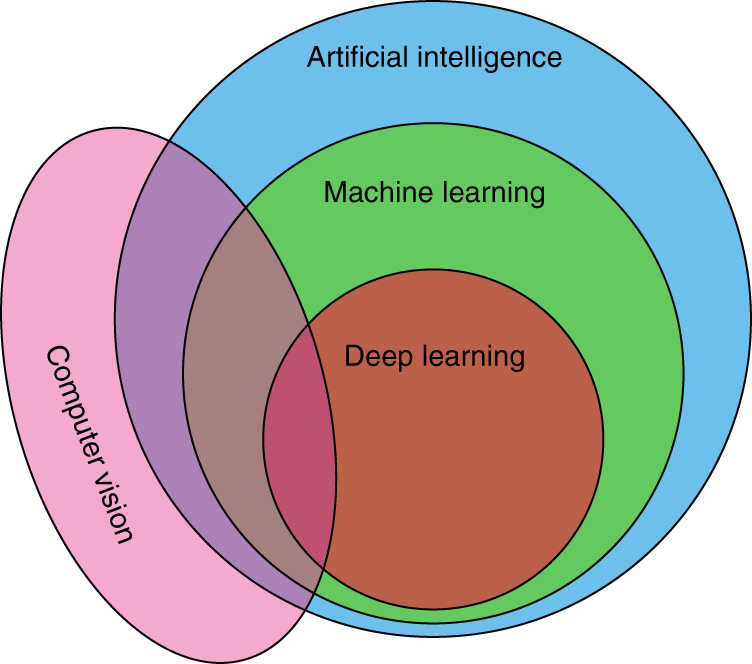
\includegraphics[width=0.75\textwidth]{resources/artificial_intelligence_set.png}
            \caption{Venn diagram of \gls{ai} and its sub-fields. Source: \cite{ruffle2018artificial}.}
            \label{fig:image_classification}
        \end{figure}
    
    \subsection{Machine learning}
        While \gls{ai} is a broader concept, \gls{ml} is the core part of it. It focuses on algorithms that can access data and learn from it automatically without human intervention, which is based on the assumption that we should give machines access to information and let them learn from it themselves.
        
        \Gls{ml} is sometimes considered difficult to understand. However, the basic intuition is not that complicated. At its core, we can imagine that \gls{ml} algorithm is just searching a decision hyperplane of best fit in many dimensions. If we have up to 2-D feature space of the problem, we can even visualize the split and the results. That is why dimensionality reduction such as \gls{pca} \cite{pearson1901liii} is often used.
        
        The complexity in the machine learning tasks is the training and preparation of the training dataset. There is a great emphasis on the flawlessness of the dataset because if it contains errors, the algorithm can quickly learn these imperfections and thus decrease the generalization performance. 
        
        There are three main \gls{ml} categories presented below that are being actively researched. They differ from each other in the way they handle data, but also with the outputs they provide.
        
        \begin{figure}[h]
            \centering
            \subfloat[]{{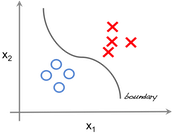
\includegraphics[width=3.8cm]{resources/supervised_learning.png} }}
            \qquad
            \subfloat[]{{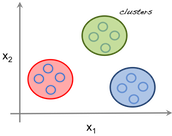
\includegraphics[width=3.8cm]{resources/unsupervised_learning.png} }}
            \qquad
            \subfloat[]{{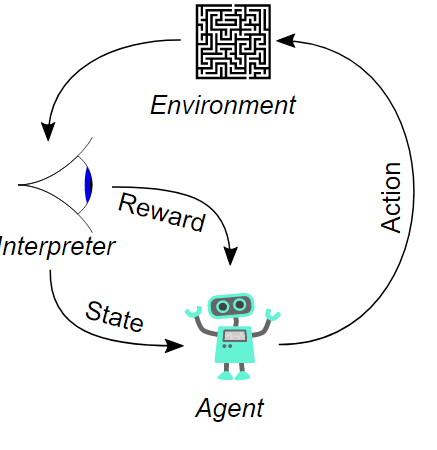
\includegraphics[width=3.4cm]{resources/reinforcement_learning.png} }}
            \caption{Categories of machine learning tasks. a) Supervised learning. b) Unsupervised learning. c) Reinforcement learning. Source: \cite{kuramasupervisedunsupervised, wiki:reinforcementlearning}}.
            \label{fig:ml categories}
        \end{figure}
        
        \subsubsection{Supervised learning}
            In supervised learning, the algorithm focuses on building a mathematical model from a set of available data that contains both the inputs and also the desired outputs. The most common example is to predict house prices based on various features such as the number of rooms, square floor feet, lot area, general condition, etc. \Gls{ml} model takes these features as input and based on its internal parameters, it produces output price prediction. This type of supervised learning is called regression. It is characterized by that the output is continuous value. 
            
            Another type of supervised learning is classification which is used when the outputs are restricted to a limited set of values. We could consider a simple classification problem as identification of spam emails based on its content. The output prediction for this task would be of either "spam" or "not spam." A traditional supervised classification model used for decades is a \gls{svm} \cite{cortes1995support}, that divides the data into regions separated by a linear boundary. 
            
            There is also popular sub-category called semi-supervised learning that emphasizes on using incomplete data during training, in terms of missing labels for some data samples.
         
        \subsubsection{Unsupervised learning}
            Unsupervised learning algorithms try to build a mathematical model to find patterns in data. The data given to the unsupervised model in training phase contains only input features and no desired output labels. Algorithms are then left to themselves to explore and discover critical structures in the data and group the inputs into clusters (categories). In the previous example with houses, the model would be able to find similar houses for input parameters, but not to predict the price of a given house.
            
            Typical algorithm representatives in unsupervised learning are hierarchical clustering \cite{johnson1967hierarchical}, k-means \cite{macqueen1967some}, and DBSCAN \cite{ester1996density}.

            
        \subsubsection{Reinforcement learning}
            In reinforcement learning, a mathematical model (also called agent) is given feedback in the form of positive or negative reward for his actions in a dynamic environment. Given the agent's and environment's states, the agent only takes actions which will maximize his reward or will explore a new possibility. Results of these actions are then fed back into the agent and environment, and based on that they will change their state. This step is repeated many times to improve the agent's behavior for future decisions. 
            
            Examples of rewards can be winning a game, scoring more points or earning more money. Thus it fits well dynamic tasks. Reinforcement learning, especially with deep neural network extension \cite{franccois2018introduction}, already performs well on a small human-involved task such as playing Atari games and it presents current state-of-the-art results in this field.
       
    \subsection{Deep learning}
        \Gls{dl} is a specialized form of \gls{ml} and it is currently the cutting edge of what machines can do - it has far surpassed any previous traditional algorithms for classification of images, text, and voice and we can find its use in all current machine learning applications. The essential advantage is that unlike \gls{ml} models, \Gls{dl} models are trained by large labeled sets of data where the model architecture learns the domain features directly without the need for manual feature extraction. This is also known as "end-to-end learning" where a model is given data, optimization criteria, a task to perform and it learns how to solve this task automatically. Another important fact is that today's \gls{dl} models often continue to improve as the size of the data increases.
        
        \Gls{dl} tasks can be categorized into the same categories as \gls{ml} - supervised, unsupervised, and reinforcement learning. The most common \gls{dl} models are based on an artificial neural network, which is why deep learning models are often referred to as deep neural networks. Unlike traditional neural networks with a few hidden layers, deep networks can have hundreds of layers.
        
        Although many \gls{dl} concepts such as neural networks, backpropagation, gradient descent had been around for decades \cite{fukushima1980neocognitron, lecun1989backpropagation, lecun1998gradient}, some researches asses that victory of Krizhevsky in October 2012 ImageNet competition started the "deep learning revolution" \cite{russakovsky2015imagenet}. However, it was not the only big break that happened, for example, Google’s Deep reinforcement learning based AlphaGo beating the best Go player in the world \cite{kochgo} also had a great impact on the research community. 
        
        There are two main drawbacks while using \gls{dl} architectures. Firstly, it requires a large amount of labeled data which is an even bigger problem in critical applications. In an example such as autonomous driving, it is often required to have thousands of hours of video, which can take up a few petabytes of storage space. Secondly, \gls{dl} requires substantial computing power, which is most often achieved by using high-performance \gls{gpu}s that have parallel architecture. However, most people, especially researchers, do not have their \gls{gpu} cluster, so they use cloud computing that enables them to reduce training time from weeks to hours. There are also many criticism concerns around \gls{dl} because methods are often looked at as a block box with the lack of theory, where most confirmations are done empirically rather than theoretically.
        
    \subsection{Computer vision}
        \Gls{cv} is the process of using computers to process, understand and analyze various types of image data in order to produce numerical or symbolic information, e.g., in the forms of decisions. The motivation is to automate tasks that human visual systems can do to utilize human resources on more critical tasks. Moreover, with a large number of surveillance cameras, it is not possible to monitor all of them by people. 
        
        \begin{figure}[ht]
            \centering
            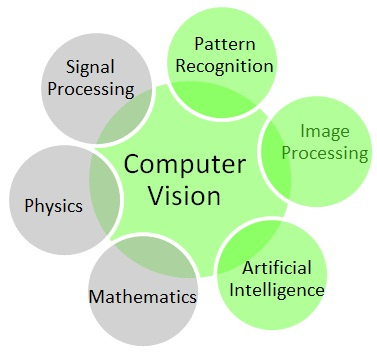
\includegraphics[width=0.55\textwidth]{resources/computer-vision-venn.png}
            \caption{Venn diagram of related fields of \gls{cv}. Source: \cite{khandelwalcv}}.
            \label{fig:convolutional neural netwok}
        \end{figure}
        
        The whole process of deciding over imagery data is called a \gls{cv} pipeline. The traditional pipeline starts with image acquisition, followed by image preprocessing and feature extraction step, ending with a classifier. This pipeline follows well-established principles from any \gls{ml} task. Hence we do not consider it necessary to explain it in this work, but we provide a reference to \cite{koenpieline} which offers a detailed description of each step.
    
        The analyzed image data can be a standard photo or video sequence from a common \gls{rgb} camera, but also to more complex data such as multi-camera video sequence and multi-dimensional imagery from satellite or medical equipment. Computers interpret this visual content very straightforwardly - as a series of pixels that forms a matrix, where each pixel has its own set of color values (see Fig. \ref{fig:lincon_pixels}). However, in order for the machines to make decisions, they need to understand higher-level concepts in the data, not to use just plain pixel values. For this reason, and also because the size of the imagery data is large, feature extraction is a common technique to obtain high-level features, thus helping computers to understand the visual context. 
        
        \begin{figure}[h]
            \centering
            \subfloat[]{{
\includegraphics[width=3.5cm]{resources/lincoln_pixel_values_1.png} }}
            \qquad
            \subfloat[]{{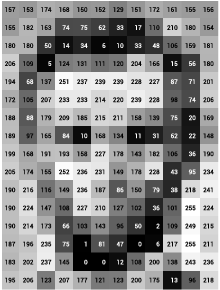
\includegraphics[width=3.5cm]{resources/lincoln_pixel_values_2.png} }}
            \qquad
            \subfloat[]{{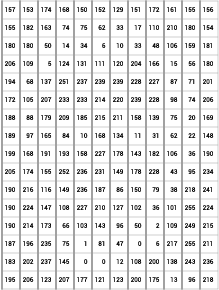
\includegraphics[width=3.5cm]{resources/lincoln_pixel_values_3.png} }}
            \caption{Pixel data diagram of simplified grayscale image demonstrating the semantic gap. a) The image itself. b) The pixels labeled with values from 0 to 255, representing their brightness. c) Pixel numbers by themselves. Source: \cite{computervisiongolan}}.
            \label{fig:lincon_pixels}
        \end{figure}
        
        To this date, we can observe two main approaches in \gls{cv} pipelines - hand-crafted \gls{ml} methods and \gls{dl} methods. The main difference is how features are obtained before they are fed into a classifier. We can think of mean, variance, median, min, and max of our data as useful measures for discrimination of samples, but since these features are specified explicitly, they are called hand-crafted. In practice, we have more complicated tasks that require more sophisticated statistical functions and feature extractors such as Haar \cite{viola2001rapid}, \gls{lbp} \cite{ojala2002multiresolution}, \gls{hog} \cite{dalal2005histograms}, \gls{sift} \cite{lowe2004method}, \gls{surf} \cite{bay2006surf}, but the idea is the same - we know how the features will look like in advance. In \gls{dl}, we know nothing about the features until we learn them from data itself. We still need to specify model and its parameters, but the real feature learning is achieved by an iterative optimization process.
        
        \Gls{cv} is nowadays ubiquitous in our society. It is used in applications such as image understanding, medicine, self-driving cars, augmented reality, and drones and there are many sub-domains of \gls{cv} that are actively researched. The most significant interest is currently on scene reconstruction, object detection and tracking, human pose estimation, and style transfer. It may be a surprise, but the core of many applications often builds upon something simple as image classification, and while many types of \gls{cv} algorithms have been around since the 1960s, recent developments in computing capabilities have driven significant improvements in how well machines understand the image content. Furthermore, with the advent of \gls{dl} approaches, \gls{cv} is becoming increasingly popular, and at the same time, there is a noticeable increase in the accuracy of many existing \gls{cv} applications. 
     
\section{Computer vision approaches}
    Because the \gls{cv} field has massively transformed into \gls{dl} algorithms, we present a brief overview of some conventional approaches that are used for solving today's \gls{cv} tasks.
    
    \subsection{Artificial neural network}
        \Gls{ann}, or simply \gls{nn} in this context, is an interconnected graph of artificial neurons that uses computational model for solving \gls{ml} tasks. In more practical terms, \gls{nn} are non-linear statistical data modeling or decision making tools that can be used to model complex relationships between inputs and outputs or to find patterns in data. In most cases, a \gls{nn} adapts its internal structure based on information that flows through the network. Thanks to many breakthrough results in recent years, it generated much excitement in the research community. 
        
        \subsubsection{Artificial neuron}
            There are many types of \gls{nn}s. However, the most researched and utilized is a particular type known as the \gls{mlp}. Its basic unit of computation is called neuron (or node). It receives input from other neurons and computes an output value. Each input $x_i$ of a neuron has its a particular weight $w_i$ value associated. The weight can be understood as relative importance to other neuron inputs. Weights and inputs are added together in weighted sum and additional bias parameter $b$ is used as a correction. In the end, activation function $\varphi$ is used to generate an output of the neuron $y_k$.  In mathematical notation, the output of a neuron is given by:
    
            \begin{equation}
                y_k = \varphi \left(\sum\limits_{j=1}^n w_j x_j + b \right)
            \end{equation}
        
        \subsubsection{Activation function}
            Since most of the real world data are non-linear, the activation function must be non-linear too. This is also very important for Universal approximation theorem \cite{hornik1989multilayer}, which says that a \gls{mlp} can approximate any function, i.e., can in principle learn anything. 
            
            To this date, many activation functions were proposed, but the most commonly known are:
            
           \begin{itemize}
                \item \textbf{Sigmoid} - The sigmoid non-linearity squashes real numbers to range between $[0,1]$.
                
                \begin{equation}
                   \sigma(x) = \frac{1}{1 + e^{-x}}
                \end{equation}
                
                \item \textbf{tanh} - The tanh non-linearity squashes real numbers to range between $[-1,1]$.
                
                \begin{equation}
                    \tanh(x) =  2\sigma(2x) - 1
                \end{equation}
                
                \item \textbf{ReLU} - The activation value of ReLU is simply thresholded at zero. As the ReLU has proved to work very well, several other variants such as Leaky ReLU, ELU, and SELU have emerged.
                
                \begin{equation}
                    f(x) = \max(0, x)
                \end{equation}
            \end{itemize}
    
            The activation function selection is crucial for task accuracy and performance. However, their thorough description is very comprehensive. Thus we recommend \cite{cs231n} for their detailed overview.

        \subsubsection{Feed-forward neural network}
            Feed-forward \gls{nn} contains multiple neurons arranged in layers. Nodes from adjacent layers have connections between them, and all these connections have associated weights. In this type of network, the information moves only in the forward direction, hence the name. No cycles are allowed in this architecture.
            
            A feed-forward \gls{nn} can consist of three types of layers:
            
            \begin{itemize}
                \item \textbf{Input layer} - The input layer is always at the beginning of the network. It provides information from outside of the model to the network. No computation is performed at this stage, and values are just passed to further neurons.
                \item \textbf{Hidden layer} - Neurons in this layer perform computations to output nodes based on input nodes and internal parameters. A feed-forward network can have zero or multiple hidden layers.
                \item \textbf{Output layer} - This layer is responsible for transferring the computed information from the network to the outside world. The transferred information usually represent a class probability score or some real-valued prediction.
            \end{itemize}
           
            The weights in neurons are iteratively improved in the training phase, where data is forwarded through the network,  then the difference between ground-truth and the predicted value is calculated. The procedure to improve the weights is known as backpropagation \cite{hecht1992theory}.  An example of a feed-forward neural network is shown in Fig. \ref{fig:neuron and neural network}. Feed-forward \gls{nn} with many hidden layers is called deep \gls{nn}.

            \begin{figure}[ht]
                \centering
                \subfloat[]{{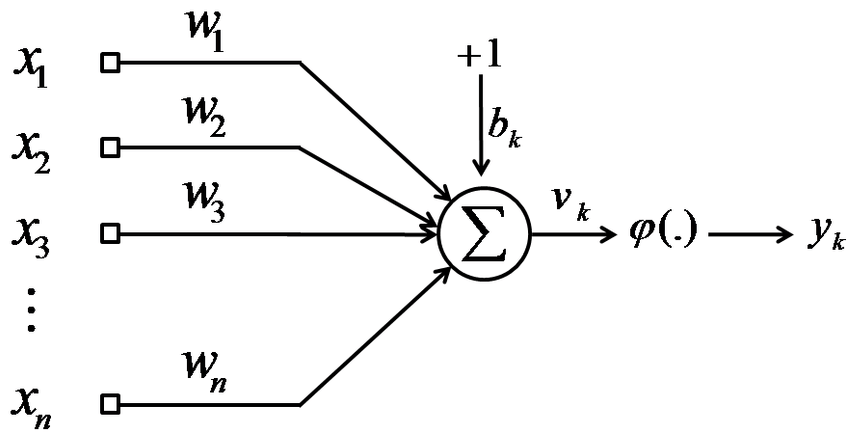
\includegraphics[width=0.35\textwidth]{resources/single_neuron.png} }}
                \qquad
                \subfloat[]{{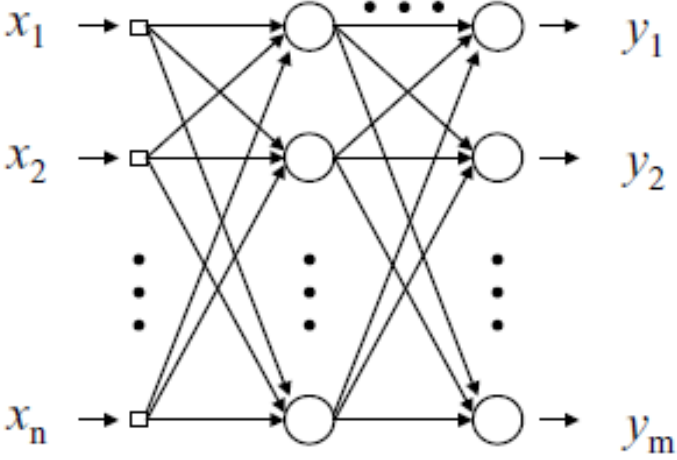
\includegraphics[width=0.35\textwidth]{resources/neural_network.png} }}
                \caption{Pixel data diagram of simplified grayscale image. a) Schematic of a single neuron. b) Schematic of a feed-forward neural network. Source: \cite{nnfurtado}}.
                \label{fig:neuron and neural network}
            \end{figure}
            
    \subsection{Convolutional neural network}
        One of the most common methods for solving computer vision task is \gls{cnn}. It uses convolutional layers to learn features from input data without minimal preprocessing. Therefore, it eliminates the need for manual feature extraction as in traditional methods. The features are learned while the \gls{cnn} trains on large labeled image dataset. This approach has shown to be highly accurate since it outperforms humans in image recognition task \cite{russakovsky2015imagenet} and it is is one of the most popular techniques for deep learning. Current applications such as object self-driving cars, object detection, medical image classification, combined with advances in GPUs and parallel computing, heavily relies on \gls{cnn} architectures. 

        A \gls{cnn} can have tens to hundreds of layers that each learn to detect different patterns or features of an image. Depth of the \gls{cnn} is critical component for a good performance \cite{russakovsky2015imagenet}. Since there is the explicit assumption that the inputs are grid-like topology, such as an image, certain properties are encoded into layer architecture that makes the forward function more efficient by reducing the number of parameters in the network. Network layers perform operations that alter the data with the intent of learning features specific to the data. 
        
        Three of the most critical layers are convolution, activation, and pooling which are often applied multiple times in a row before concluding the process of feature extraction. The goal of repetition is to identify different features, and the argument for this is the observation that images contain hierarchical structure (e.g., faces are made up of eyes, which are made up of edges, etc.), so several layers of processing will increase in extracted features complexity to features that uniquely define particular object. The outputs of this whole process are then often passed into a fully connected layer for final output, i.e., class score probabilities. 
        
        Layout, number, and type of layers form the architecture of the \gls{cnn}. To this date, dozens of architectures were proposed, and the most famous are LeNet, AlexNet, VGGNet, Inception, ResNet, ResNeXt, and DenseNet. Since each of these architectures would require extensive description, we consider it as out of the scope of this thesis, and we suggest \cite{cs231n, dascnnoverview, jordancnnoverview} for further reading. 

        \begin{figure}[ht]
            \centering
            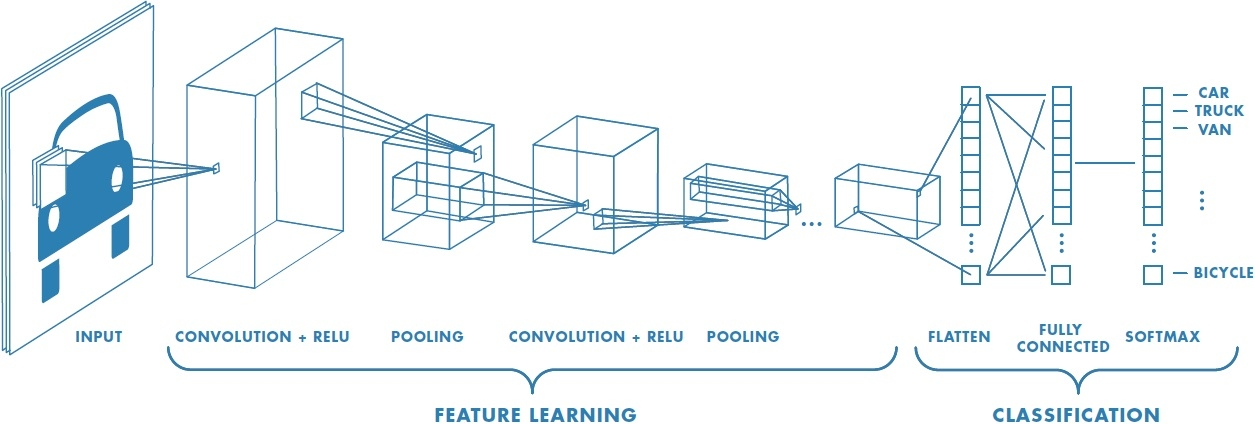
\includegraphics[width=0.85\textwidth]{resources/convolutional-neural-network.png}
            \caption{Example of a network with many convolutional layers. Filters are applied to each training image at different resolutions, and the output of each convolved image is used as the input to the next layer. Source: \cite{mathworkscnn}}.
            \label{fig:convolutional neural netwok}
        \end{figure}
        
        \subsubsection{Convolution layer}
            The convolution layer is the core building block of any \gls{cnn}, where the input image pixels are modified by a convolutional filter, which is a matrix that is multiplied with different parts of the input image. The filter is spatially smaller than an image (e.g., 3x3, 5x5, 8x8), but is more in-depth. Each filter aims to activate certain features from the images. The output of this layer is known as a feature map (alternatively activation map), and it is usually smaller in size but has more dimensions. Theoretically, a feature map will be less redundant and more informative than the original input.
            
        \subsubsection{Activation layer}
            The purpose of this layer is the same as in the \gls{ann}, to introduce non-linearity in the feature maps. Favorite choice in the \gls{cnn} case is ReLU due to its simplicity which implies an effective training process.
            
        \subsubsection{Pooling layer}
            Since the convolutional layer expands dimensionality, pooling is a process that reduces the size of the feature map by a factor of whatever size is pooled. The consequence is the reduction of the number of parameters that the network needs to learn. The input image is scanned over each dimension by a sliding window and either the max, sum or average the window is taken as a representation of that portion of the image. 
            
        \subsubsection{Fully-connected layer}
            A fully-connected layer is most often the last layer of the \gls{cnn} architecture. It is implemented as a common feed-forward \gls{nn} with fixed input size. Adding this type of layer usually helps with combining the high-level features from convolutional layers into a non-linear function. A frequent choice of fully-connected layer output type is a vector that contains the probabilities of each object class of an image being classified.

    \subsection{Transfer Learning}
        It is sporadic for people to train an entire \gls{cnn} from scratch. There are three main reasons for this. Firstly, it has been proved that \gls{cnn} and \gls{nn} are very sensitive to proper weights initialization. Many works have been done on this topic, and it is generally not recommended to use random or zero initialization since it can lead to several problems during training. Secondly, there are very few datasets with sufficient size. Using only a tiny dataset will lead to insufficient accuracy or overfitting. Lastly, the training phase is computationally intensive. Modern \gls{cnn} architectures can take a few weeks to train on multiple \gls{gpu}s properly.

        In practice, it is common to take pre-trained parameters from existing \gls{cnn} used for a similar task (e.g., ImageNet classification \cite{russakovsky2015imagenet}, which contains 1.2 million images with 1000 categories) and use them as initialization or a fixed feature extractor for the task of interest. This use of existing \gls{cnn} as a feature extractor is straight-forward because only the last fully-connected layer needs to be removed or replaced.
        
\section{Computer vision tasks}
    In this section, we provide a quick overview of tasks relevant to the thesis topic and their specific challenges. Since the first early steps of computer vision field in the 1960s, the scientists tried to build camera robots with intelligent behavior. However, it turned out to be a much more complex problem than they initially thought and as a first step, they desired to extract 3-D structure from 2-D images to achieve full scene understanding. Therefore, forming the very first computer vision task - scene reconstruction. Moreover, it was this time, that many feature extraction algorithms that are popular today were founded, including edge detector and lines extractors. 
    
    Later, the robots, which partially understood the scene, needed to move around while avoiding obstacles, which could be accomplished through motion analysis. Some existing algorithms such as Kalman filter already existed. Hence they were adapted to \gls{cv} field. However, motion detection algorithms such as optical flow and background subtraction methods have also been developed.
    
    In recent years, there is a significant advance in this field, and we can finally see the real applications of these robots which are, for example, self-driving cars. As a result, today's most considerable emphasis is on feature-based methods used together with machine learning algorithms to produce numerical or symbolic information for decision making. However, it should be noted that many algorithms still come from the research done in early beginnings. 
    
    \begin{figure}[ht]
        \centering
        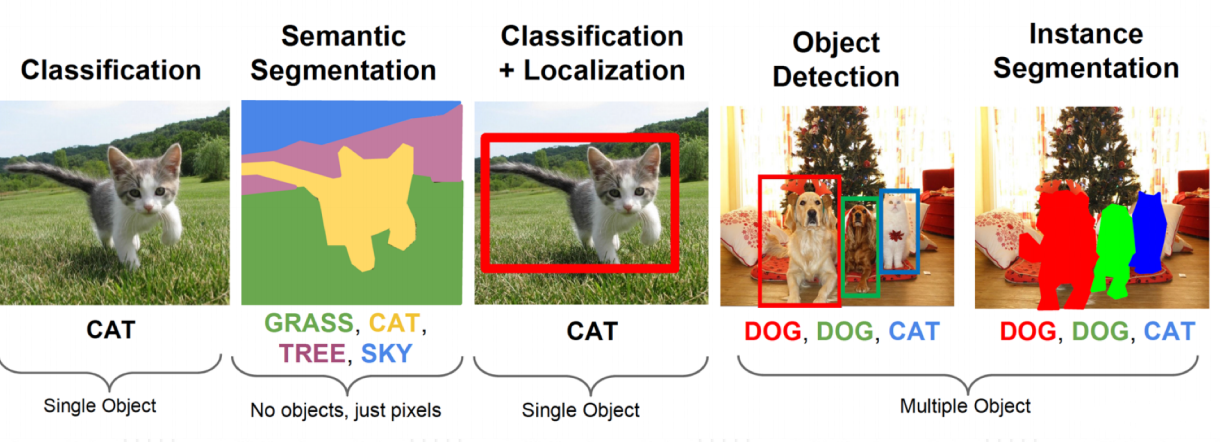
\includegraphics[width=0.95\textwidth]{resources/computer-vision-tasks.png}
        \caption{\Gls{cv} tasks that are most popular nowadays. Source: \cite{cs231n}.}
        \label{fig:computer-vision-tasks}
    \end{figure}
    
    
    \subsection{Camera calibration}\label{camera_calibration}
        Cameras and other sensors with optics have been with us for decades. Recently they became part of our everyday life which can be demonstrated, for example, by finding it on every phone or laptop. However, these cameras have one big drawback caused by their easy availability and cheap purchase price. Their image is distorted considerably. Fortunately, the distortion can be described by mathematical equations and can, therefore, be partially or entirely removed. 
        
        To deal with the distortion, the camera calibration technique is most often employed. It is the process of finding the intrinsic and extrinsic parameters of arbitrary camera setup. The intrinsic parameters deal with the internal characteristics of the camera and lens combination. The extrinsic parameters refer to the 3D orientation and position of the camera in the space. Example of intrinsic parameters is the focal length, principal point, sensor skew. With knowledge of intrinsic parameters, it is possible to establish a relation between image pixels and real-world units to do real-world measurements and also remove lens distortion, which degrades image quality. 
        
        Two essential types of distortion exist. First is radial distortion that causes straight lines to appear curved. It becomes larger the farther points are from the center of the frame. The other one is tangential distortion caused by the lens not parallel to the image plane. Before running any critical \gls{cv} application, both distortions need to be corrected first. 
        
        The radial distortion can be represented as follows:

        \begin{align}
            x_{distorted} = x( 1 + k_1 r^2 + k_2 r^4 + k_3 r^6) \\ 
            y_{distorted} = y( 1 + k_1 r^2 + k_2 r^4 + k_3 r^6),
        \end{align}
        and tangential as follows:
        \begin{align}
            x_{distorted} = x + [ 2p_1xy + p_2(r^2+2x^2)] \\
            y_{distorted} = y + [ p_1(r^2+ 2y^2)+ 2p_2xy],
        \end{align}
        where $x, y$ are coordinates of the original point, $x_{distorted}, y_{distorted}$ are their distorted projections, and $k_1, k_2, k_3, p_1, p_2$ are unknown distortion coefficients. These coefficients do not depend on the scene viewed and they remain the same regardless of the captured image resolution.
        
        To find these coefficients, we must provide several images of predefined and well-known pattern to camera calibration framework. Generally, it is recommended to use at least ten images of the pattern from different angles. The framework then detects specific points in the image of which relative positions are known. Based on these image coordinates and their relative correspondence in the real world, it is possible to solve for distortion coefficients. A standard pattern used in camera calibration is a chess board with square corners as target points. For a more detailed description of this technique, we recommend \cite{zhang1999flexible}.

    \subsection{3-D scene reconstruction}
        3-D reconstruction is the process of obtaining 3-D information from the captured 2-D scene. It is a complicated process by the fact that in the imaging process the depth of the space is lost. To solve this task, stereo vision or methods based on triangulation with multiple captured images from different angles are often employed. However, some single-view approaches are sufficient to obtain a partial or complete reconstruction, and for the scope of this thesis, they are the most relevant.
        
        Single-view approaches might be further categorized into calibrated and uncalibrated methods. Calibrated ones use parameters obtained by camera calibration presented in \ref{camera_calibration}, and their main disadvantage is that internal camera parameters may not always be constant. The intrinsic parameters may be affected by environment effects or only by changing a focal length. Proposals for the calibrated methods can be found in \cite{orteu1997camera, wilczkowiak2001camera, kushal2002simple}.
        
        On the other hand, algorithms developed for uncalibrated scenarios require no knowledge of the camera's intrinsic and extrinsic parameters. The use of known scene constraints replaces camera calibration. These constraints include planarity of points, the parallelism of lines, and parallelism of points. Therefore, no scene markers or specialized sensors are required; these cues are inferred directly from the captured 2-D image, which leads to flexible algorithms that can be applied to a wide range of scenarios. One of the most famous works in this field is \cite{criminisi2012accurate}.

        Further, the discipline that deals with estimating real-world measurements in 2-D image scenes is known as single-view metrology. The groundbreaking work in this field is \cite{criminisi2002single}.
        
    \subsection{Motion analysis}
        As a result of access to a massive amount of video data, motion analysis has drawn considerable interest in recent times. Its main goal is to output information based on the apparent motion in the sequential images. The information produced often depends on neighboring images and is related to specific time-point. 

        Motion analysis is a field that has been researched since the 1970s, but since then, the algorithms, approaches, and also disciplines has changed. Most proposed methods are based on pixel displacements of underlying physical points. The simplest representative in this field is an optical flow algorithm that detects motion. Nowadays we are more likely to encounter more complex frameworks used in the task such as human motion analysis, scene behavioral analysis, and surveillance tracking.
        
        In the context of tracking, motion information is mostly employed as one of the features that are used during the matching step between new and previously tracked objects. Modern motion filters also allow us to predict movement information of objects even if no motion information is available in multiple frames. Examples of well-used motion filters are particle filter, and Kalman Filter and its non-linear variants. Their thorough comparison can be found in \cite{labbe2015kalman}.
  
    \subsection{Image classification}
        The typical problem in computer vision field is that of determining if image data contain a specific object. Image classification, with its main component known as classifier, is a particular application of computer vision which assigns an input image one label from a fixed set of categories. The general approach is to assign probabilities for each class and then choose the most likely one. Despite its simplicity, it is one of the core problems in computer vision with a large variety of applications. Moreover, many other distinct computer vision tasks (localization, object detection, segmentation, etc.) can be reduced to image classification.
        
        In Fig. \ref{fig:image_classification}, we can see the image of a cat with associated probabilities of belonging into four categories. We need to keep in mind that in this figure, the image is represented as a large 3-dimensional matrix of numbers in a computer's memory. In this case, the image is 248 pixels wide, 400 pixels tall, and has three color channels. Therefore, the image consists of $248 \times 400 \times 3$ numbers, or a total of $297 600$ numbers. Each number is an integer that ranges from 0 (black) to 255 (white). To conclude, Therefore, the task is to turn a quarter of a million numbers into a single label, such as cat. \cite{cs231n}
        
        \begin{figure}[ht]
            \centering
            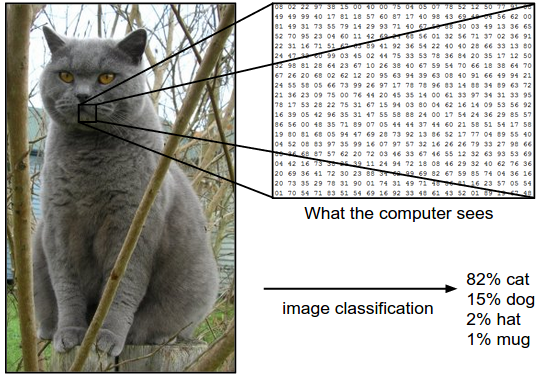
\includegraphics[width=0.75\textwidth]{resources/image_classification.png}
            \caption{Image classification example. Source: \cite{cs231n}.}
            \label{fig:image_classification}
        \end{figure}
    
        Since this task of recognizing objects is relatively trivial for humans, it only makes sense to consider challenges for \gls{cv} algorithms. The challenges are visualized in Fig. \ref{fig:image_classification_challenges} and they are especially:
    
        \begin{itemize}
            \item \textbf{Viewpoint variation} - A single instance of an object can be oriented in many ways concerning the camera.
            \item \textbf{Scale variation} - Visual classes often exhibit variation in their size (size in the real world, not only in terms of their extent in the image).
            \item \textbf{Deformation} - Many objects of interest are not rigid bodies and can be deformed in extreme ways.
            \item \textbf{Occlusion} - The objects of interest can be occluded. Sometimes only a small portion of an object could be visible.
            \item \textbf{Illumination conditions} - The effects of illumination are drastic on the pixel level.
            \item \textbf{Background clutter} - The objects of interest may blend into their environment, making them hard to identify.
            \item \textbf{Intra-class variation} - The classes of interest can often be relatively broad, such as a chair. There are many different types of these objects, each with their appearance.
        \end{itemize}
        
        \begin{figure}[ht]
            \centering
            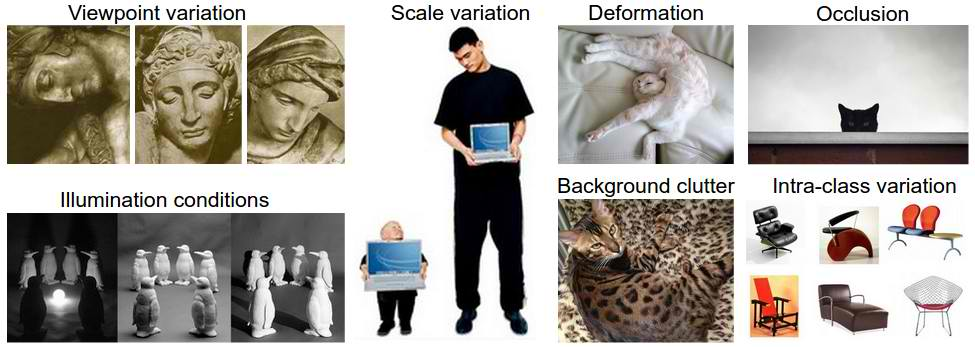
\includegraphics[width=0.85\textwidth]{resources/image_classification_challenges.png}
            \caption{Image classification challenges. Source: \cite{cs231n}.}
            \label{fig:image_classification_challenges}
        \end{figure}
        
         A good image classification model must be invariant to the cross product of all these variations, while simultaneously retaining sensitivity to the inter-class variations. \cite{cs231n}
         
    \subsection{Object detection}
        Image classification models can classify input images into the most likely category. However, typical images including photos are usually more complex and contain multiple objects. Hence, assigning single object category does not make much sense.
        
        Object detection is a well-researched and more appropriate method that helps to identify multiple objects from predefined categories from a single image. The output of the typical object detector is an object's bounding box, category, and confidence of the detection. The bounding box patches can be then used for further visual tasks.
        
        The big break in object detectors came in 2001 with the introduction of Haar cascades by Paul Viola and Michael Jones \cite{viola2001rapid}. Their detector was able to operate in real-time and was subsequently implemented in all digital cameras. Although it could be trained to detect a variety of object classes, it was used mainly for the face detection task. 
        
        After a long time, another promising detector known as \gls{hog} \cite{dalal2005histograms} was introduced in 2005. \gls{hog} was focused on pedestrian detection in static images and was further improved for video sequences, as well as to a variety of object classes including animals and vehicles. It has been used for a long time in conjunction with other feature extractors for various detection tasks until the success of \gls{dl} architecture in 2012 ImageNet competition \cite{russakovsky2015imagenet}. Since then, the use of conventional detectors is mostly replaced with deep neural networks.
        
        In object detection based on \gls{cnn}s, there are two main core design choices. First is, hypothesize object regions and then classify them. Second, divide the image into a grid and directly predict bounding boxes with class probabilities in a single evaluation, thus only one feed-forward pass. Although a few state-of-the-art representatives for each category are briefly reviewed below we suggest \cite{huang2017speed, xuobjectdetection, ouaknineobjectdetection} for their detailed overview.
        
        \subsubsection{\Glsentryfull{r-cnn}}
            \Gls{r-cnn} \cite{girshick2016region} is very first and intuitive architecture that started the era of object detection with \gls{cnn}s. The pipeline of the model begins with scanning the input image for possible objects using Selective Search algorithm \cite{uijlings2013selective}, which generates a large number of proposals that are reduced to some reasonable amount (typically to order of thousands). Moreover, each proposal is also resized to match the input of a \gls{cnn}. Further, the \gls{cnn} is used to extract image features, and the output vector is then fed into a \gls{svm} classifier to verify if an object exists within the region. If yes, a linear regressor is used to refine the position of the bounding box.
            
            \begin{figure}[ht]
                \centering
                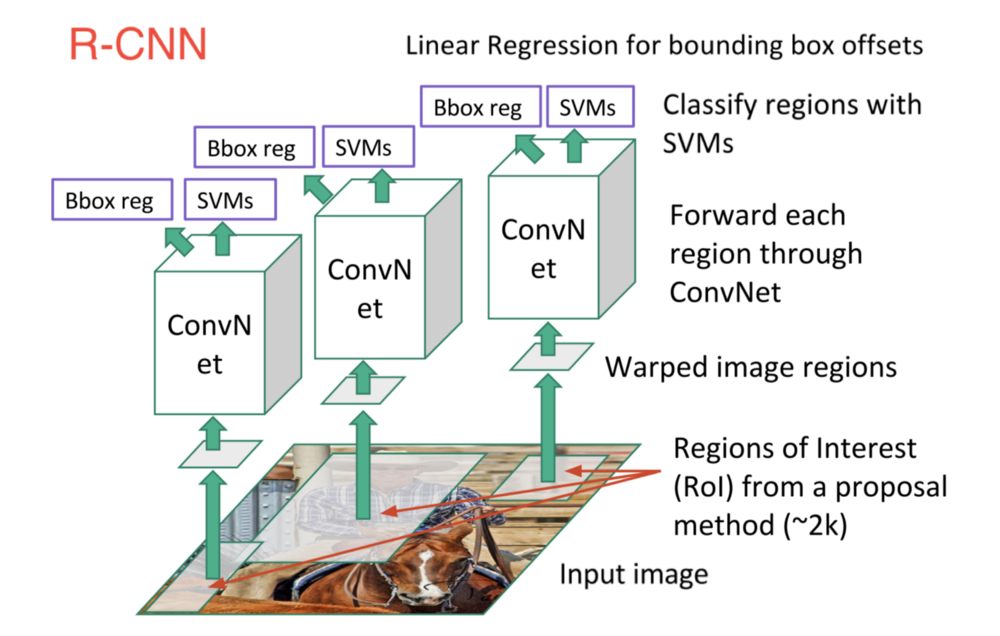
\includegraphics[width=0.85\textwidth]{resources/r_cnn_architecture.png}
                \caption{\Gls{r-cnn} architecture. Source: \cite{xuobjectdetection}.}
                \label{fig:r-cnn architecture}
            \end{figure}
        
            To sum it up, this approach turns object detection into an image classification discussed before. The drawback of this method is that the training and inference performance is very slow. For example, the inference time for a single image varies from tens of seconds to minutes.

        \subsubsection{\Glsentryfull{fast r-cnn}}
            Just year after the publication of \gls{r-cnn}, the same authors improved the approach with new \gls{fast r-cnn} \cite{girshick2015fast} architecture. It resembled the original in many ways. However, they drastically improved the training and testing speed performance.
            
            The improvement consisted of two main aspects. The feature extraction run by \gls{cnn} is no longer run thousands of time over each of the proposed regions, but only once over the entire image. The regions are still obtained by Selective search algorithm. However, its input is the feature map output of the \gls{cnn}. The proposed regions are then reshaped using an RoI pooling layer and instead of training many different \gls{svm} classifiers for each object class, there is a single fully connected \gls{nn} with softmax layer that outputs the class probabilities directly.
            
            \begin{figure}[ht]
                \centering
                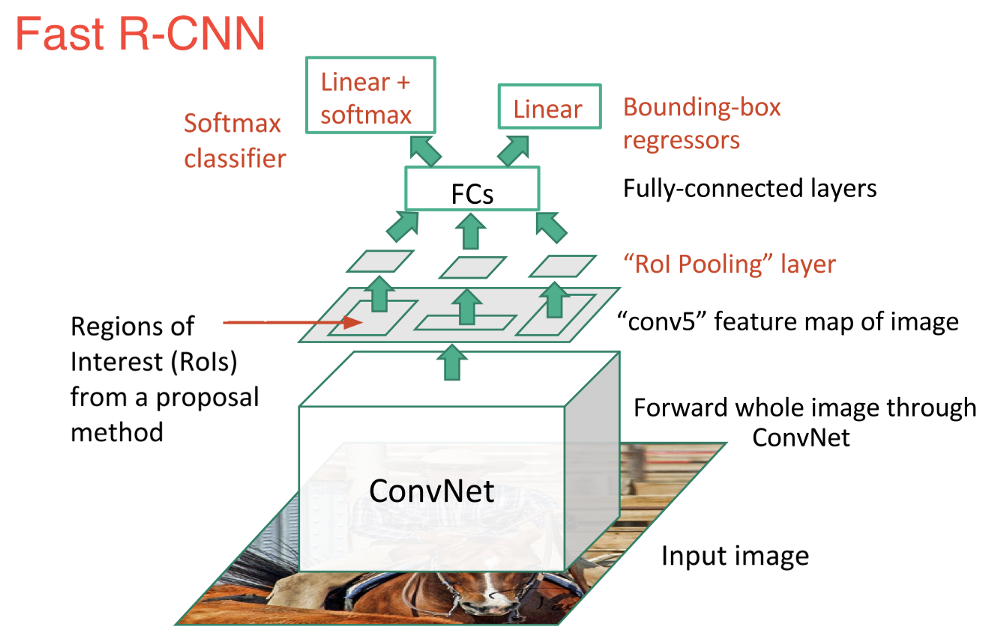
\includegraphics[width=0.85\textwidth]{resources/fast_r_cnn_architecture.png}
                \caption{\Gls{fast r-cnn} architecture. Source: \cite{xuobjectdetection}.}
                \label{fig:fast r-cnn architecture}
            \end{figure}
    
        \subsubsection{\Glsentryfull{faster r-cnn}}
            Both of the architectures mentioned above use a Selective Search algorithm to find out the region proposals. However, it turned out that Selective Search is the computational bottleneck. Besides that, it has another big disadvantage - it is a fixed algorithm; no parameter learning is happening during the training phase which may lead to bad region proposal candidates. Therefore, a new architecture know as \gls{faster r-cnn} \cite{ren2015faster} was introduced to improve these shortcomings. 
            
            \Gls{faster r-cnn} completely replaced the use of the Selective Search algorithm with a separate \gls{nn} (known as the \gls{rpn}) to identify region proposals. The \gls{rpn} is run right after the feature extraction, and once we obtain the region proposals, they are feed into what is essentially \gls{fast r-cnn}.

            \begin{figure}[ht]
                \centering
                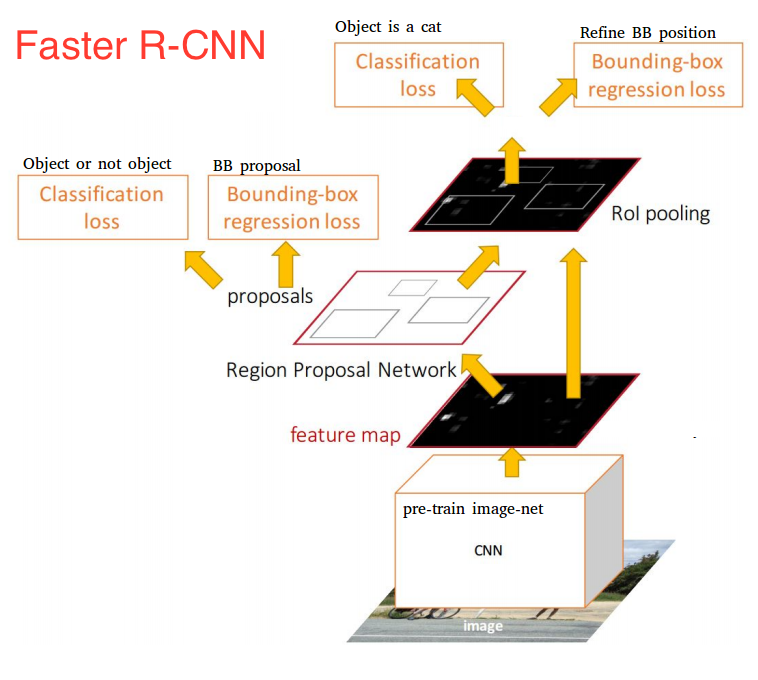
\includegraphics[width=0.85\textwidth]{resources/faster_r_cnn_architecture.png}
                \caption{\Gls{faster r-cnn} architecture. Source: \cite{xuobjectdetection}.}
                \label{fig:faster r-cnn architecture}
            \end{figure}
            
            To conclude, \gls{faster r-cnn} is combination between the \gls{rpn} and \gls{fast r-cnn}. It is much faster than its predecessors, and it can even be used for real-time object detection in a video sequence. It is still widely deployed in today's frameworks thanks to its speed and accuracy performance.
            
        \subsubsection{\Glsentryfull{yolo}}
            All of the previous object detection algorithms use proposed regions to localize the object within the image. It means that the detector does not look at the whole image. Instead, it evaluates regions which have high probabilities of containing the object. In \gls{yolo} \cite{redmon2016you}, a single \gls{cnn} directly predicts bounding boxes and class probabilities with a single forward pass.
            
            Initially, the model takes the input image and divides it into a $S \times S$ grid. Within each cell of the grid, $m$ bounding boxes are taken. For each of selected bounding box, the network outputs a class probability and refinement for the bounding box. If the bounding box has the class probability above a threshold value, it is then used to locate the object within the image. 
            
            Since the model predicts a high number of bounding boxes, the \gls{nms} \cite{rosebrocknms} procedure is applied at the end of the network to merge highly-overlapping bounding boxes of the same object into a single one.
            
             \begin{figure}[ht]
                \centering
                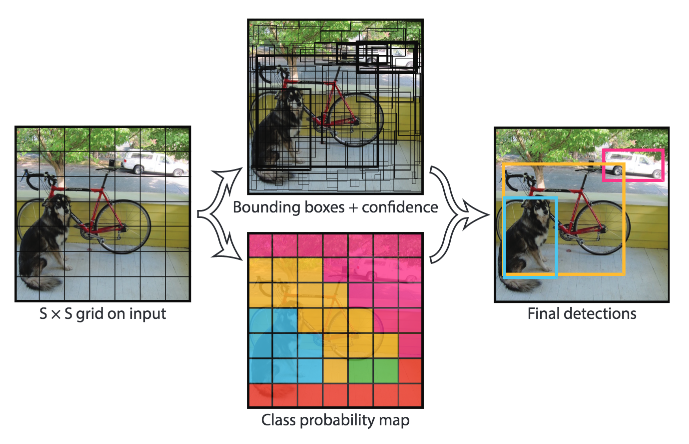
\includegraphics[width=0.85\textwidth]{resources/yolo_approach.png}
                \caption{Example of \gls{yolo} approach. Source: \cite{redmon2016you}.}
                \label{fig:yolo approach}
            \end{figure}
            
            Due to its simplicity, it is much faster than other detection algorithms mentioned. Depending on the backbone architecture, it can run approximately 15 to 150 \gls{fps}. The limitations of \gls{yolo} are that it struggles with small objects and unusual aspect ratios, which is due to the spatial constraints of the algorithm. However, the authors tried to improve this shortcoming in the newly released \gls{yolo}v3 architecture.

    \subsection{Face recognition}
        Face recognition is a prominent biometric technique that is used for everything from automatically tagging pictures on social networks to unlocking cell phones. Its main components are an object detector trained to detect face regions and classifier that embeds faces into vectors.
        
        It has been a long-standing research topic in the \gls{cv} community since it uses \gls{cv} algorithms to extract specific and distinctive information about a person's face, such as distance between the eyes, shape of the chin. This information is then converted to a compact feature vector and stored into a face database. It is desired only to include specific details that can distinguish one face from another to maintain a reasonable size of the feature vector. 
        
        Each facial feature vector can be compared to others to find the most likely match which helps to verify personal identity. However, some face recognition systems are designed to calculate a probability match score to provide several potential matches, instead of just returning a single result. The results of face recognition systems can vary under challenging conditions such as poor lighting, low resolution, improper angle of view.
        
        For decades, only traditional methods such as filtering responses, a histogram of the feature codes, or distribution of the dictionary atoms were used to recognize faces. However, these approaches were improving the accuracy very slowly and were suffering from a lack of distinctiveness and compactness. Effects of lighting, pose and expression drastically worsened the results. Fortunately, this has all changed with the advent of \gls{dl}. In 2014, DeepFace \cite{taigman2014deepface} approach achieved the state-of-the-art accuracy on the famous face recognition benchmark, approaching human performance on the unconstrained condition for the first time. This has caused this field to move in the direction of \gls{dl}, and it completely reshaped all aspects of face recognition. On Fig. \ref{fig:deep face recognition} the typical pipeline of face recognition is visualized.
        
        \begin{figure}[ht]
            \centering
            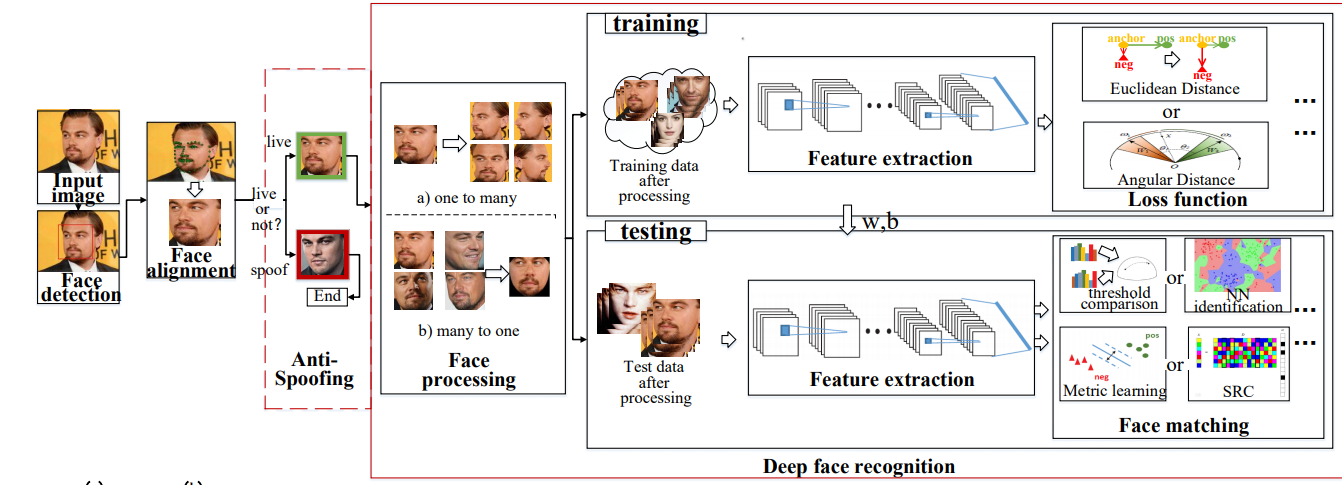
\includegraphics[width=1\textwidth]{resources/deep_face_recognition.png}
            \caption{Common pipeline for state-of-the-art face recognition systems. Source: \cite{wang2018deep}.}
            \label{fig:deep face recognition}
        \end{figure}

\section{Software frameworks}
    Research in the fields of \gls{ai} requires the use of analytical tools, technologies, and languages to help extract insights and value from data, and after that build sustainable prediction model. The key advantages of using frameworks and libraries are the ability to quickly develop and test new ideas and run efficiently on \gls{gpu}s.

    According to a 2017 survey of 16,000 data scientists by Kaggle revealed that researches in  \gls{ai} most rely on Python language \cite{mostuseddatasciencetools}. So there is no surprise that most of these packages are developed for that language. For this reason, we provide a quick overview of significant and widespread Python \gls{ml} and \gls{cv} frameworks.
    
    \subsection{OpenCV}
        OpenCV \cite{opencv_library} is a popular, cross-platform, and open-source \gls{cv} and \gls{ml} library written in C/C++ language. It was originally sponsored by Intel but now driven mostly by the open-source community with more than 47 thousand people. It has more than 2500 optimized algorithms, which includes a comprehensive set of both classic and state-of-the-art computer vision and machine learning algorithms. These algorithms can be used to detect and recognize faces, identify objects, classify human actions in videos, track camera movements, extract 3D models of objects, stitch images together, etc. OpenCV is used extensively in companies, research groups, and governmental bodies. 
        
    \subsection{TensorFlow}
        TensorFlow \cite{abadi2016tensorflow} is an open source software library for numerical computation using data flow graphs. The graph nodes represent mathematical operations, while the graph edges represent the multidimensional data arrays (tensors) that flow between them. This flexible architecture enables users to deploy computation to one or more CPUs or GPUs in a desktop, server, or mobile device without rewriting code. TensorFlow also includes TensorBoard, a data visualization toolkit.

        TensorFlow was originally developed by researchers and engineers working on the Google Brain team within Google's Machine Intelligence Research organization to conduct machine learning and deep neural networks research. The system is general enough to be applicable in a wide variety of other domains, as well.

        TensorFlow provides stable Python and C APIs as well as non-guaranteed backward compatible API's for C++, Go, Java, JavaScript, and Swift. 
        
    \subsection{PyTorch}
        PyTorch \cite{paszke2017automatic} is an open source library designed to enable rapid research on machine learning models. It builds upon a few projects, most notably Lua Torch, Chainer, and HIPS Autograd, and provides a high-performance environment with easy access to automatic differentiation of models executed on different devices (CPU and GPU). To make prototyping easier, PyTorch does not follow the symbolic approach used in many other deep learning frameworks, but focuses on differentiation of purely imperative programs, with a focus on extensibility and low overhead. 
        
    \subsection{Caffe2}
        Caffe2 \cite{caffe2} aims to provide a smooth and straightforward way for users to experiment with deep learning and leverage community contributions of new models and algorithms. Users can bring their creations to scale using the power of GPUs in the cloud or to the masses on mobile with Caffe2's cross-platform libraries. In May 2018, the development team decided to merge Caffe2 into PyTorch and make them a single package to enable a smooth transition from fast prototyping to fast execution. 
        
    \subsection{Theano}
        Theano \cite{2016arXiv160502688short} is a Python library that allows defining, optimizing, and evaluating mathematical expressions involving multi-dimensional arrays efficiently. Since its introduction in 2008, it has been one of the most used CPU and GPU mathematical compilers – especially in the machine learning community - and has shown steady performance improvements. However, the development team decided to stop further releases in 2017. 
        
\section{Evaluation metrics} \label{evaluation-metrics}
    In this section, we provide a brief overview of standard evaluation metrics relevant to the tracking field.
    
    \subsection{\Glsentryfull{iou}}
        \Gls{iou}, also known as the Jaccard index, is an evaluation metric used as a similarity measure in any object detection task. It measures the ratio between predicted and ground-truth bounding box given by:
        
        \begin{equation}
            \text{IoU} = \frac{\text{Area of overlap}}{\text{Area of union}} 
        \end{equation}
        
        The possible values for \gls{iou} are from $[0, 1]$ and their significance can be found in Fig \ref{fig:iou-examples}. \Gls{iou} is a common evaluation metric that can be found in any object detection challenge.

        \begin{figure}[ht]
            \centering
            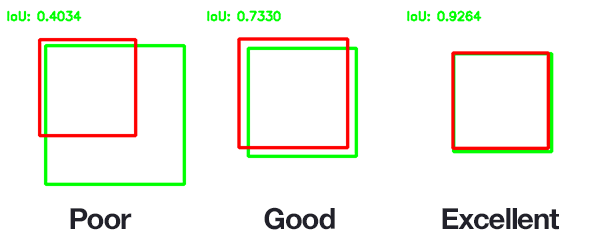
\includegraphics[width=0.95\textwidth]{resources/iou_examples.png}
            \caption{An example of computing Intersection over Unions for various bounding boxes. The predicted bounding boxes are drawn in red color, while the ground-truth ones are drawn in green color. Source: \cite{iourosebrock}.}
            \label{fig:iou-examples}
        \end{figure}
        
    \subsection{\Glsentryfull{mota}}
        The \gls{mota} is the most widely used metric for evaluating a tracker's performance. Its main advantage is expressiveness as it combines three different sources of errors:
        
        \begin{itemize}
            \item \textbf{\Gls{fp}} - The number of incorrect detections.
            \item \textbf{\Gls{fn}} - The number of missed detections.
            \item \textbf{\Gls{idsw}} - The number of identity switches.
        \end{itemize}

        The \gls{mota} equation is then given by:
        
        \begin{equation}
            \text{MOTA} = 1 - \frac{\sum_{t} \left( \text{FN}_t + \text{FP}_t + \text{IDSW}_t \right)}{\sum_{t}\text{GT}_t},
        \end{equation}
        
        where $t$ is the frame index, and GT is the number of ground-truth objects. The possible values are reported in the percentage from $(-\infty, 100]$. Negative values are possible when the number of errors made exceeds the number of all objects in sequence.
    
    \subsection{\Glsentryfull{motp}} 
        The \gls{motp} represents the average dissimilarity between the ground-truth and the predicted bounding boxes. It is calculated as 
        
        \begin{equation}
            \text{MOTP} = \frac{\sum_{t,i} d_{t,i}}{\sum_{t}c_t},
        \end{equation}
        
        where $c_t$ denotes the number of matches in frame $t$ and $d_t,i$ denotes the bounding box overlap of ground-truth and the predicted target. It thereby gives the average overlap between all correctly matched hypotheses and their respective objects and ranges between $t_d := 50\%$ and $100\%$. \cite{MOTChallenge2015}
    
    \subsection{\Glsentryfull{fps}} 
        The \gls{fps} is a common metric used in many fields to measure the run-time performance of camera equipment, algorithms, animations, rendering, etc. In this context, it expresses the ability of an algorithm to process and analyze a certain number of images per second. With increasing algorithm complexity, the frame rate decreases. Real-time ability in video sequence processing is assumed at 25 \gls{fps} \cite{MOTChallenge2015}.
    \chapter{Related work}\label{related_work}
    In this chapter, we briefly present relevant work addressing similar problems in \gls{mot} and soft-biometrics field. Given the vastness of the topic, we only limit the review to significant work.

\section{\Glsentrylong{mot}}
     Most state-of-the-art algorithms addressing \gls{mot} follow the tracking-by-detection approach, which heavily relies on the performance of the underlying object detector. However, the trend is now shifting to the end-to-end learning solutions and constructing stronger similarity scores based on appearance, motion, and interaction cues. Although recent \gls{nn} based detectors have outperformed all other methods for object detection \cite{russakovsky2015imagenet, ren2015faster, redmon2016you}, \gls{mot} remains a challenging and popular topic.
   
    \Gls{sort} \cite{bewley2016simple} is the first pragmatic approach where the main focus is to associate objects efficiently for online and real-time applications. They showed that the quality of detections plays a crucial role in tracking performance and according to their experiments, they can improve tracking by almost 20 \%, depending on the detector. Despite using an only simple combination of standard techniques as the Kalman Filter for motion prediction and Hungarian algorithm for the association of the tracks, they were able to achieve comparable performance to other state-of-the-art online trackers. 
    
    By adding a deep association metric to \gls{sort} \cite{wojke2017simple}, it was successfully integrated with the appearance model that improves the tracking performance. The appearance model is based on \gls{cnn} trained on large scale person \gls{reid} dataset. Due to this extension, the algorithm can track objects through longer periods of occlusion, effectively reducing the number of identity switches. The framework of this paper is used for our tracking task. Thus it is more explained in the next chapter. 

    In 2016, revolutionary end-to-end learning approach based on \gls{rnn} \cite{mikolov2010recurrent} has been introduced in a novel \cite{milan2017online}. Their proposed \gls{lstm} \cite{hochreiter1997long} architecture is capable of performing all multi-target tracking tasks including prediction, data association, state update as well as initiation and termination of targets within a unified network structure. One of the main advantages of this approach is that it is completely model-free, i.e., it does not require any prior knowledge about target dynamics, clutter distributions, etc. However, the object detections should be given as input.
    
    It was not the only case of successful use of \gls{rnn}. In the paper \cite{sadeghian2017tracking} published year later, a new approach combining multiple cues such as appearance, movement, and interaction is proposed. These cues are fed into \gls{lstm} \cite{hochreiter1997long} architecture, which learns and remembers the dependencies in a sequence of observation, in contrast to pairwise similarity where only the observations from the current and previous frames are used. Their proposed framework follows end-to-end fashion, and their architecture does not require object detections as input.
    
    Competitive tracking results can be achieved even without sophisticated tracking methods. Tractor \cite{DBLP:journals/corr/abs-1903-05625} accomplishes tracking without following the common tracking-by-detection approach and authors performed no training or optimization on tracking data. Instead, they exploited the bounding box regression of an object detector to perform temporal realignment and to predict the position of an object in the next frame. They also provide a simple extension to this approach, in the form of Siamese \gls{nn} for \gls{reid} and motion analysis model, which achieve state-of-the-art performance on tracking benchmarks. 
    
    Results of recent tracking evaluations show that bounding box tracking performance is saturating \cite{mot16}. Further improvements will only be possible when moving to the pixel level., which is a reason why the authors of recent 2019 work \cite{DBLP:journals/corr/abs-1902-03604} are expanding from \gls{mot} to \gls{mots}. They propose new TrackR-CNN baseline method which jointly addresses detection, tracking, and segmentation with a single convolutional network that extends Mask R-CNN architecture with 3D convolutions to incorporate temporal information, and by an association head which is used to link object identities over time. They also provide evaluation metrics and new dataset with masks for over one thousand distinct objects in ten thousand frames. The main advantage of \gls{mots} is that segmentation based tracking results, are by definition non-overlapping and can thus be compared to ground truth straightforwardly.
    
\section{Soft-biometrics}
    There has not been much written about the general use of biometrics in retail yet. However, some exceptions exist. For example, in \cite{fookes2010semi} authors propose semi-supervised intelligent multi-camera surveillance framework that can perform multiple tasks, including camera management, camera calibration, and multi-view object tracking with \gls{reid} based on appearance soft-biometric traits. The survey \cite{quintana2016improving} from 2016 provides a complete overview of innovative camera approaches that can be applied in the retail environment. The study \cite{de2018comparative} aims at recognizing the age, gender, presence of eyeglasses and beard of passers-by in a retail store. Their solution lies in custom \gls{cnn} architecture that extracts these traits.
    
    Although end-to-end solution targeting solely retail environment have not been proposed yet, there are plenty of works that deal only with certain soft-biometric features.
   
    \subsection{Body traits}
        Frequent body traits \cite{de2018comparative} extracted from an \gls{rgb} camera are height, gait, and color of clothes. The best feature for distinctiveness between individuals proved to be gait, which is the reason why it is often used in forensic analysis. However, there are not many uses for gait in the retail environment. Thus we only focus on others.
        
        \subsubsection{Height estimation}
            There has been a long history in determining an individual's height. One of the essential works in this field is \cite{criminisi2002single}, where authors proved that height estimation is possible without any information about camera parameters, only several scene correspondences with known real-world measurements are sufficient. In their work, they also describe how the affine 3D geometry of a scene can be reconstructed from a single image.
            
            In \cite{viswanath2009simplified} authors describe a simple uncalibrated model of error distribution in height as a function of the location of the object in the image and the estimated camera height. Their approach builds on previous work \cite{criminisi2002single} and improves the accuracy in estimating the height while reducing the burden of reliably computing the ground plane. 
        
            More recent work \cite{momeni2012height} uses a single calibrated camera, more explicitly assuming the knowledge about its pose concerning the world and vanishing point in the reference direction. According to their proposed theorem, by knowing the proportion of camera height concerning the object height, at the object’s position in the image plane, it is possible to estimate the height of the object in the real world. Their presented method gives accurate results in unstructured environments, regardless of the relative distance from the camera.
            
            Authors of \cite{li2015simplified} proposed a framework utilizing the calibrated camera for estimating height in video surveillance. Their primary assumption is that it is possible to obtain a camera's focal length, tilting angle, and height by using non-linear regression model from the observer's head and foot points of people in the scene, instead of estimating the vanishing point and vanishing line. Once these calibration parameters of a camera are obtained, the physical height of a person can be estimated from a pair of head and foot points observed from the image and their proposed formula.

        \subsubsection{Color clothes estimation}
            One of the essential works \cite{yamaguchi2012parsing} in this field comes from 2012, where authors focus on fashion photographs and propose an effective method to produce intricate and accurate parse of a person’s outfit. They also introduced large labeled dataset with available labeling tools. Finally, they designed a prototype application for visual garment search.
            
            DeepFashion \cite{liu2016deepfashion} is another large-scale clothes dataset with extensive annotations introduced in 2016. Authors also introduced a new baseline method, namely FashionNet, which learns clothing features by jointly predicting clothing attributes and landmarks. The estimated landmarks are then employed to pool or gate the learned features. 
            
            The current state-of-the-art is the baseline model built upon Mask R-CNN \cite{he2017mask}, termed Match R-CNN \cite{ge2019deepfashion2}. The authors of this work also proposed new challenging large-scale dataset DeepFashion2. Their presented model offers end-to-end training framework that jointly learns clothes detection, landmark estimation, instance segmentation, and consumer-to-shop retrieval. 

    \subsection{Facial traits}
        If we focus only on the head of individuals, then many algorithms targeting facial biometric \cite{wang2018deep} are regularly introduced. Most of the work from this field comes inevitably from face recognition task, which is natural since this field has a history almost as long as fingerprint recognition. Commonly extracted facial soft-biometrics are gender, ethnicity, age, emotion, pose, glasses, beard, and mustache with a frequent goal to explore their discrimination capabilities among other individuals during in-the-wild scenarios. We will limit this review to only the most important ones that can be used for retail use, namely age, gender, emotion, and pose \cite{balaban2015deep}. Some of these traits are commonly estimated together by using one model.
        
        \subsubsection{Multi-task approaches}
            In paper \cite{yin2018multi}, authors propose multi-task \gls{cnn} for face recognition where identity classification is the main task and pose, illumination, and expression estimations are the side tasks. They also provide analysis of multi-task learning with extensive experiments that demonstrate the effectiveness of the proposed approach.
            
            HyperFace \cite{ranjan2019hyperface} is an algorithm that can simultaneously do face detection, landmarks localization, pose estimation and gender recognition. It uses \gls{cnn} model architecture that fuses intermediate layers of a \gls{cnn} using a separate \gls{cnn} followed by a multi-task learning algorithm that operates on the fused features. It exploits the synergy among the tasks which boosts up their performances. They also proposed two variants with a different focus -- HyperFace-ResNet that achieves high accuracy and Fast-HyperFace that significantly improves the speed of the algorithm. Their experiments show that the proposed models can capture both global and local information in faces and perform significantly better than many competitive algorithms for each of these four tasks.
            
            The authors of the same composition later released improved version \cite{ranjan2017all} that can additionally solve for tasks of smile detection, age estimation, and face recognition. They also extended their approach by training the model on multiple datasets whereas HyperFace was trained only on one. 

        \subsubsection{Age and gender estimation}\label{age_and_gender_estimation_related}
            In most retail cases, we are interested in estimating age at the same time as gender \cite{ranjan2017all, wang2015deeply}, since these traits play a crucial role in targeted advertising. In the case of age, it is very challenging to obtain it by the camera because the apparent age sometimes significantly differ from the real one. Fortunately, particular numbers are not that important, but instead categories such as child, youth, adult, middle-age and elderly. On the other hand with gender, the situation is slightly simpler because there are several other attributes that algorithms can use. We further present only recent proposals from this field that mostly relies on \gls{dl} models. 
            
            The first ever work applying \gls{dl} methods was presented by the authors in \cite{wang2015deeply}. They propose a \gls{cnn}-based framework for age estimation, and instead of using only the feature map obtained at the top layer, they utilize feature maps obtained in different layers for the final estimation. Additionally, they incorporate a manifold learning algorithm in the proposed scheme, and that significantly improves the performance.

            In the same year, work \cite{rothe2015dex} introduced \gls{dex} method that tackles the estimation of apparent age in face images. They proposed \gls{cnn} with VGG-16 architecture pre-trained on ImageNet. They also introduced large-scale face images dataset with available age to pre-train their \gls{cnn}. 

            Recently in 2019, authors of \cite{yang2018ssr} proposed \gls{ssr}, a light-weight \gls{cnn} model with real-time performance that is targeting age and gender estimation. Their work is inspired by DEX, and they address age estimation by performing multi-class classification and then turning classification results into regression by calculating the expected values. Their greatest benefit is the compactness of the model presented. \Glsentryshort{ssr} takes only 0.32 MB of memory, and despite its size, it is approaching the performance of more than 1500× larger state-of-the-art methods.
            
        \subsubsection{Facial expression recognition}
            Facial expression \cite{goodfellow2013challenges} is one of the main clues that can be utilized in retail stores to measure the satisfaction of the consumers. \cite{arriaga2017real} is a very popular paper that proposes a general \gls{cnn} framework with real-time performance. Their model is capable of accomplishing the tasks of face detection, gender classification, and emotion classification simultaneously in one blended step using the proposed architecture. They validate their results on recent datasets, but also by building their robot which succeeded in the competition. Their architecture and pre-trained models are released under an open-source license.

            The framework known as EmoPy \cite{emopy} is a toolkit with multiple implemented \gls{cnn} architectures for emotion recognition. For example, they use time-delayed 3-D \gls{cnn}  that utilizes temporal information as part of its training samples. In other words, instead of using an only single image for prediction, it uses past images from a series for additional context. The idea is to capture the progression of a facial expression leading up to a peak emotion. They also propose hybrid \gls{lstm} \cite{hochreiter1997long} architecture that combines approaches from \gls{cnn} and \gls{rnn} to include temporal context from whole still images, not only from face patches as the former presented. They also introduce a simpler model trained on FER2013 dataset \cite{goodfellow2013challenges} which can make predictions based on a single image. Moreover, in their framework, it is possible to specify only a smaller subset of all seven emotions available, which is undoubtedly more practical in real-world scenarios.
            
            Paper \cite{zeng2018facial} from 2018 has presented a novel approach for facial expression recognition using \gls{dsae} \cite{sun2016sparse}, which can automatically distinguish the expressions with high accuracy. Both the facial geometric and appearance features have been introduced to compose a high-dimensional feature with accurate and comprehensive information of emotions. In the end, the experiment results have demonstrated that the proposed approach outperforms the other three state-of-the-art methods by a large margin.
             
        \subsubsection{Head pose estimation}
            Head pose estimation \cite{wang2018deep} is closely related to other facial analysis problems, and it might be useful in a retail store when there is a requirement for modeling customer attention on specific products or areas. Traditional algorithms work by estimating facial landmarks (key points) from the target face and then solving the 2D to 3D correspondence problem with a mean human head model as a reference. Since it is a very fragile method that relies on landmark detection performance, current state-of-the-art methods focus on detecting the pose without detecting the key points. 
            
            In 2018, an accurate and easy to use head pose estimation \gls{cnn} known as Hopenet \cite{Ruiz_2018_CVPR_Workshops} was introduced. In their work, authors can detect intrinsic Euler angles (yaw, pitch, and roll) directly from image intensities through joint binned pose classification and regression. They showed their network generalization capacity by testing the performance on various external datasets without fine-tuning. 
        
            A novel method is known as FSA-Net \cite{fsanet} also targets head pose estimation. Authors of this work proposed a light-weight non-landmark \gls{cnn} model that even outperforms methods utilizing multi-modality information from depth and \gls{rgb} cameras.
    \chapter{Design}
    \chapter{Implementation}
    This chapter contains information related to the implementation of the proposed framework. The whole implementation is done in Python language with the dependence on several other frameworks and libraries, including OpenCV, Tensorflow, and Darknet. The main application functionality spans eight Python modules.
    
\section{Module tracking\textunderscore app}
    This module is the main entry point of the application. It contains only one essential function that is responsible for running the proposed framework. In this function, we first load the input image stream, calibration parameters and other components such as object detectors, feature extractors, tracker, and image viewer. Then there is a loop that runs the algorithms as long as input frames are available. The application can be run either from an IDE or from the command line with various input parameters.

\section{Module detection}
    The detection module contains multiple wrappers for various object and face detectors proposed in \ref{detection_and_tracking_components}. It is responsible for loading these models based on input parameters, detecting objects in the input frame, and filtering detections by input criteria. 

\section{Module feature\textunderscore extraction}
    In this module, we propose to interface and pre-processing to various appearance feature extractors including age, gender, and emotion models, but also height estimator. The module also contains a function that assigns face regions to people bounding boxes.

\section{Module kalman\textunderscore filter}
    This module is vital for the proposed motion analysis method because it contains the configuration of the utilized filter. Our approach uses Kalman Filter implementation from famous FilterPy \cite{labbe2015kalman} library. The module is also responsible for converting filter's internal state to visualizable bounding box and for converting measurements to filter's input.

\section{Module matching}
    The matching module contains an efficient implementation of a proposed distance metric, namely the cosine metric for appearance (section \ref{appearance_metric}) and enhanced Euclidean distance for the state (section \ref{state_metric}). Metrics are calculated by NumPy, which is a high-performance linear algebra library written in C language. To make the computations as efficient as possible, we utilize the NumPy broadcasting technique.

\section{Module tracking}
    In the tracking module, we propose PeopleTracker class that is responsible for the actual matching of detections and tracks. It is mostly inspired by code from \cite{wojke2017simple}, but some modifications in the matching algorithm were made. Successfully matched tracks are updated from here, and unmatched detections are transformed to tentative tracks.
    
\section{Module track}
    An instance of Person class from the track module represents a single person that was detected in the scene. Each person instance has set of attributes including id, color for visualization, status, creation frame number, time since the last update, age in frame units, last body bounding box, last face bounding box, Kalman filter instance, and dictionary with gathered features.
    
\section{Module output\textunderscore statistics}
    This module is responsible for transforming all possible data to brief output statistics. It includes a class TrackingEvaluator which evaluates the tracking performance of the algorithm based on provided annotations. Class OutputStatistics is responsible for converting gathered data about people to usable outputs.

\section{Module visualization}
    Visualization module contains all drawing related functions including plotting output graphs using Matplotlib and Seaborn libraries. It implements an ImageViewer class that is responsible for showing the preview of processed images. The ImageViewer class also contains functionality that allows easier debugging by allowing users to pause the algorithm or process the stream by one frame at a time.
    \chapter{Evaluation}
%Further work
    \begin{conclusion}
    This work was focused on building a framework for the task of people tracking and soft-biometric data extraction. In the introductory chapter, we thoroughly described the assignment with sufficient motivation, but also with its challenges. In the following theoretical chapter, we have described the necessary theoretical background in detail for understanding of this thesis. In chapter \ref{related_work}, we briefly reviewed the existing solutions, and based on that some popular methods were implemented from scratch or customized from open-source repositories to meet the thesis goals. The implemented solution is then evaluated in the evaluation chapter, and further improvements are proposed. The result is a functioning people tracking and soft-biometrics extracting framework that can be deployed in a real-world application.
    
    According to the table \ref{table:tracking_results}, the proposed algorithms achieve {state-of-the-art} results in long-term people tracking. The best solution based on \gls{faster r-cnn} achieves only two identity switches on our dataset, which is an outstanding outcome. The quality of the detected boxes is also very high. Evaluated height and age estimators achieve exact results. However, in future work, it is necessary to evaluate more individuals.
    
    The proposed methods are designed in several variations to meet different trade-offs of accuracy versus computational expensiveness, and since the final design of the framework is fully modular, it can be easily configured to meet demands for various other scenarios. We put much effort into the application design as a whole so that it can be easily expanded and it can now be deployed in real-world applications. There are still some shortcomings in the framework, but they are described so that they can be further worked on and we hope that this work will be a useful as a starting point for other people interested in this topic. 

\end{conclusion}
    
    % bibliography
    \bibliographystyle{prefs/iso690}
    \bibliography{ref}
    
    \appendix
    
    % acronyms
    \printglossaries
    
    % media contents
    \chapter{Media contents}\label{app:CDcontent}
    \begin{figure}
    % 	\dirtree{%
    % 		.1 readme.txt\DTcomment{the file with CD contents description}.
    % 		.1 data\DTcomment{the data files directory}.
    % 		.2 graphs\DTcomment{the directory of graphs of experiments}.
    % 		.3 *.eps\DTcomment{the B/W graphs}.
    % 		.3 *.png\DTcomment{the color graphs}.
    % 		.3 *.dat\DTcomment{the graphs data files}.
    % 		.1 exe\DTcomment{the directory with executable WBDCM program}.
    % 		.2 wbdcm\DTcomment{the WBDCM program executable (UNIX)}.
    % 		.2 wbdcm.exe\DTcomment{the WBDCM program executable (Windows)}.
    % 		.1 src\DTcomment{the directory of source codes}.
    % 		.2 wbdcm\DTcomment{the directory of WBDCM program}.
    % 		.3 Makefile\DTcomment{the makefile of WBDCM program (UNIX)}.
    % 		.2 thesis\DTcomment{the directory of \LaTeX{} source codes of the thesis}.
    % 		.3 figures\DTcomment{the thesis figures directory}.
    % 		.3 *.tex\DTcomment{the \LaTeX{} source code files of the thesis}.
    % 		.1 text\DTcomment{the thesis text directory}.
    % 		.2 thesis.pdf\DTcomment{the Diploma thesis in PDF format}.
    % 		.2 thesis.ps\DTcomment{the Diploma thesis in PS format}.
    % 	}
    \end{figure}
    

\end{document}
